%!TEX root = ../main.tex

\chapter{Search strategy}
The previous chapter presented the method for localizing sources of ionizing radiation.
%Given the collected measurements, it can compute the maximum likelihood estimate of the sources locations.
To increase the accuracy of such estimate, the \ac{UAV}s should collect as many measurements.
The nature of the measurements (as stated before, the emission as well as the detection process are stochastic processes and the intensity of radioactive emission decreases with inverse square law as the distance from source grows) 
requires the \ac{UAV}s to fly as close as possible to the currently most likely source estimates to either confirm or disprove the presence of the radioactive source at the given position.
Moreover, the sensitivity computed in the \ac{MLEM} method provides information about how much has been the area explored by the compton cameras onboard the \ac{UAV}s.

This motivates the search strategy described in this section:
The movement of the \ac{UAV}s should be controlled in a way that they simultaneously perform the following tasks:
\begin{itemize}
  \item \textbf{exploration} - explore the least explored maps in the area of interest and increase the chance that so far unobserved sources of radiation will be detected
  \item \textbf{exploitation} - fly where the radioactive sources are likely present (based on the current maximum likelihood estimate) to improve the accuracy of the estimate. 
\end{itemize}




%The maximum likelihood approach requires collecting as many measurements as possible to make the estimate more accurate.
%At the same time, the drones should explore the unexplored area to increase chance that the estimation method won't miss any source of ionizing radiation.
%The task for the mutirobotic system can be summarized as follows:
%\begin{itemize}
%  \item \textbf{exploration} - explore the least explored maps in the area of interest
%  \item \textbf{exploitation} - acquire more measurements from areas, where the source of ionizing radiation is likely present
%\end{itemize}

\begin{figure}[!h]

  \subfloat[\textbf{generated waypoints}] {
    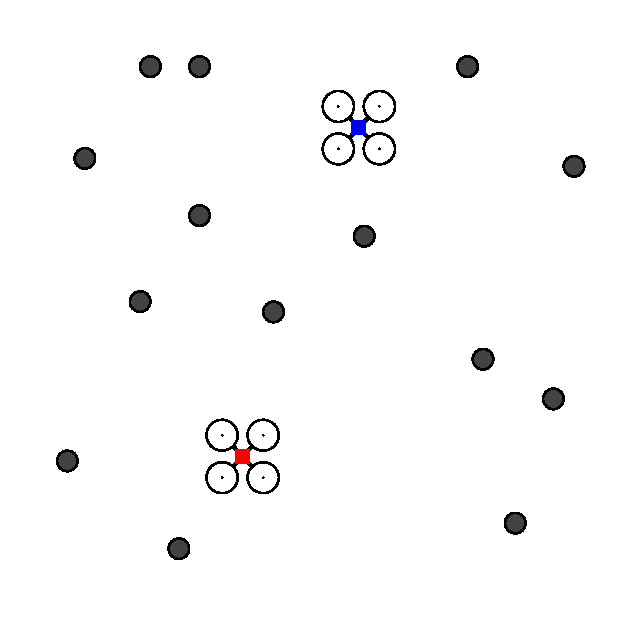
\includegraphics[width=0.3\textwidth]{./fig/photos/pip1.eps}

    \label{fig:pip1}
  }
  \subfloat[\textbf{weighting and filtering}] {
    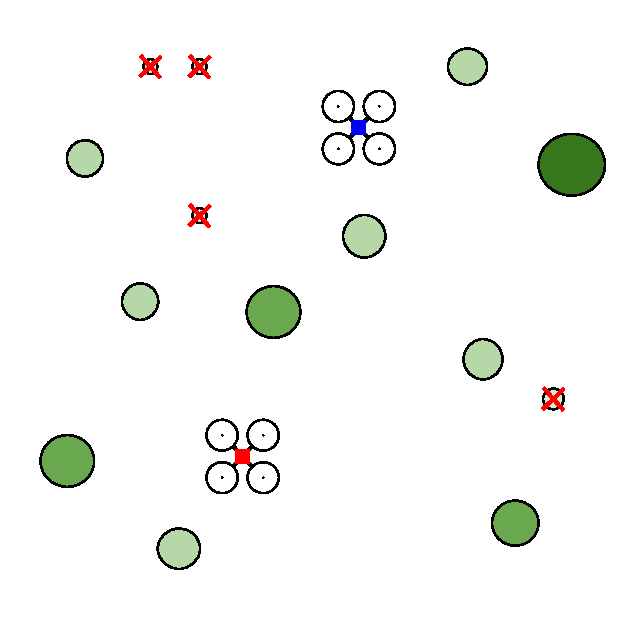
\includegraphics[width=0.3\textwidth]{./fig/photos/pip2.eps}
    \label{fig:pip2}
  }
  \subfloat[\textbf{clustering}] {
    \includegraphics[width=0.3\textwidth]{./fig/photos/pip3.eps}
    \label{fig:pip3}
  }
  \newline
  \subfloat[\textbf{filtering recently visited waypoints}] {
    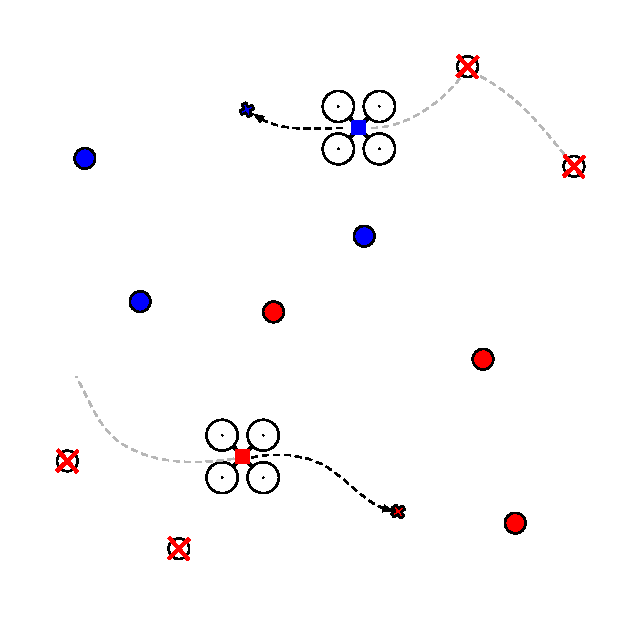
\includegraphics[width=0.3\textwidth]{./fig/photos/pip4.eps}
    \label{fig:pip4}
  }
  \subfloat[\textbf{task assignment}] {
    \includegraphics[width=0.3\textwidth]{./fig/photos/pip5.eps}
    \label{fig:pip5}
  }
  \subfloat[\textbf{path planning}] {
    \includegraphics[width=0.3\textwidth]{./fig/photos/pip6.eps}
    \label{fig:pip6}
  }
  \caption{Individual steps of the system pipeline.}
  \label{fig:pipeline}
\end{figure}

\section{Waypoints generation, weighting and filtering}
The current estimate of ionizing radiation sources positions serves as an input for the waypoint generation method.
The map estimated by the \ac{MLEM} method is processed and local maxima of the map are found.
The map position is taken as local maxima if there is no map position with higher expected emission rate in it's neighborhood.

\section{Clustering}
The generated waypoints need to be assigned to the individual \ac{UAV}s. 
First step for this is clustering it into groups, one for each \ac{UAV}.
Clustering belongs to the group of unsupervised machine learning methods.
The goal of clustering is to partition the data into distinct groups (clusters), where data points within the same cluster are more similar to each other than to those in other clusters.
The euclidean distance is the measure of similarity used in this scenario.
The clustering algorithm of choice for the given task is \textbf{KMeans}, originally described in \cite{kmeans}.

\subsection{KMeans algorithm}
The basic euclidean version of KMeans is defined as follows:
Let's denote data points to be clustered as $\{\mathbf{w}_{1}, \mathbf{w}_{2}, \dots , \mathbf{w}_{n}\}$.
The task is to assign each of the data points into one of the $k$ clusters, $\{C_{1}, C_{2}, \dots, C_{k}\}$.
Each cluster is represented by its centroid, $\mathbf{c}_{1}, \mathbf{c}_{2}, \dots, \mathbf{c}_{k}$.
The criterion function that should be minimized is then formulated as
\begin{equation}
  J = \sum_{i = 1}^{k} \sum_{\mathbf{w} \in C_{i}} \| \mathbf{w} - \mathbf{c}_{i} \|^{2}.
\end{equation}
In other words, we want to find such clusters so that the sum of distances between data points and corresponding centroids of clusters will be minimal.
\textbf{KMeans} is an iterative algorithm.
In each iteration, it assigns each data point to the nearest centroid based on the euclidean distance. 
After all data points are assigned to clusters, the centroids are updated by calculating the mean of all data points in each cluster. 
These two steps are repeated until convergence.
It is important to note that the outcome of the algorithm depends on the initialization of centroids and the method converge to local minima based on that initialization.

\subsection{Constrained KMeans and initialization}
For the purpose of assigning waypoints to the \ac{UAV}s, the optimality of the solution is not required.
However, we would like to assign waypoints to the \ac{UAV} that are in it's neighborhood.
Moreover, we would like to guarantee that each \ac{UAV} has at least one point assigned (the standard version of KMeans does not guarantee non-emptiness of the clusters).
Therefore the constrained variant of KMeans (described in \cite{constrained_kmeans}) is used.
The centroids are initialized at the future positions of the \ac{UAV}s.





\section{Filtering recently visited waypoints}
The following assumption is made:
to acquire more measurements from different sides and localize the sources more precisely, it is better to keep the \ac{UAV}s in motion, better then statically measure radiation at certaion position for longer time.
Therefore are prioritized the waypoints that were not recently explored by any of the \ac{UAV}s (meaning that no \ac{UAV} was in a close proximity of the sensor in past seconds).
For that purpose, we define short-term sensitivity matrix $\mathbf{\hat{S}}$, which is independent of the sensitivity matrix $\mathbf{\hat{S}}$ defined in \ref{eq:sen_iter}, 
although it is computed analogically.

Same as before, the matrix $\mathbf{\hat{S}}^{[0]}$ is initialized with zeros.
Lets denote $V^{[n:n+1]}$ the set of viewpoints that were newly sampled after update step $n$ and needs to be processed. 
The short-term sensitivity matrix $\mathbf{\hat{S}}^{[n+1]}$ with elements $\hat{s}_{j}^{[n+1]}$ is computed as:
\begin{equation}
  \hat{s}_{j}^{[n+1]} = \alpha \hat{s}_{j}^{[n]} + \sum_{v \in V^{[n:n+1]}} s_{jv} \Delta_{v}. 
  \label{eq:sen_iter_shortterm}
\end{equation}
We may notice that the only difference between short-term sensitivity equation \ref{eq:sen_iter_shortterm} and sensitivity equation \ref{eq:sen_iter} is that new scaling parameter $\alpha \in [0, 1)$ was added.
The $\alpha$ can be named as a forgetting factor.
It scales past $\hat{s}_{j}$ values with some non-negative $<1$ number, making newly sampled viewpoints more important.








%%%%%%%%%%%%%%%%%%%%%%%
%%% TASK ASSIGNMENT %%%
%%%%%%%%%%%%%%%%%%%%%%%
\section{Task assignment}

After assigning all waypoints into clusters, the optimal sequence of waypoints inside the cluster should be determined.

\subsection{Travelling salesman problem}
The \ac{TSP} is a classical problem in computer science. 
The problem can be formulated as follows: 
A complete oriented graph is given, where $V$ (set of vertices) represent locations that should be visited and $E$ (set of edges) represents the distances between then vertices.
The task is to find the path through the vertices (find a Hamiltonian cycle), so that each vertex is visited exactly once, the starting and ending point are the same and the distance of the path (the sum of weights assigned to the edges involved in the path) is minimal.
The edges of the graph are typically stored in a distance matrix $\mathbf{D}\in \mathbb{R}^{\left|V\right|\times\left|V\right|}$, where $d_{ab} \in \mathbf{D}$ represents the distance from vertex $a$ to vertex $b$.

\subsection{Problem modifications}
The problem of finding the optimal sequence of waypoints $\{v_{1}, v_{2}, \dots , v_{n}\}$ for an \ac{UAV} is transformed to the travelling salesman problem and solved using LKH solver\footnote{available at: http://webhotel4.ruc.dk/~keld/research/LKH/}.
However, we require some additional features, not only finding the minimal Hamiltonian cycle in the graph with respect to the euclidean distances between waypoints.
The starting vertex of the sequence should be the future position of the drone, let's denote it as vertex $v_{0}$.
Secondly, the path of the \ac{UAV} should not end in the starting vertex $v_{0}$, the last point of the sequence can be any of the waypoints $\{v_{1}, v_{2}, \dots, v_{n}\}$.
Because of that, we introduce dummy vertex denoted as $v_{F}$.
We formulate the transformed problem as follows.
The set of vertices of the graph is $\{v_{0}, v_{1}, v_{2}, \dots,v_{n}, v_{F}\} \in V$, where: 
\begin{itemize}
  \item $v_{0}$ is the starting point of the optimal sequence of waypoints
  \item $v_{1}, v_{2}, \dots, v_{n}$ are the points to be visited by the \ac{UAV} and   
  \item $v_{F}$ is the dummy vertex that serves as the last point of any sequence found by the solver.
\end{itemize}

The distance matrix $\mathbf{D}$ of euclidean distances between each pair of $\{v_{0}, v_{1}, v_{2}, \dots,v_{n},  v_{F}\}$ 

\begin{equation}
  \mathbf{D}_{eukl} = 
  \begin{pmatrix}
    0 & d_{0,1} & d_{0,2} & \dots & d_{0, n} & d_{1, F} \\
    d_{1,0} & 0 & d_{1,2} & \dots & d_{1, n} & d_{2, F} \\
    d_{2,0} & d_{2,1} & 0       & \dots & d_{2, n} & d_{3, F} \\
    \dots&\dots & \dots & \dots & \dots & \dots \\
    d_{n,0}& d_{n, 1} & d_{n, 2} & \dots & 0 & d_{n, F} \\
    d_{F, 0} & d_{F,1} & d_{F,2} & \dots & d_{F, n} & 0 
\end{pmatrix}
\end{equation}
is then modified in the following way:
a positive constant $M$ is introduced (it holds that $M>10\mathrm{max}(d),  \forall d \in \mathbf{D}_{eukl}$).
The purpose of this constant is to forbid some edges in the graph so that they couldn't be chosen by the numerical solver.
We set to $M$ all edges that connects the dummy vertex $v_{F}$ with all vertices $\{v_{1},v_{2}, \dots, v_{n}\}$, because we require the vertex $v_{F}$ to be the last one in the optimal sequence.
Additionally, the edge weight connecting the starting point $v_{0}$ and $v_{F}$ is also set to $M$.
Furthermore, the distance from any vertex $\{v_{1}, v_{2}, \dots, v_{n}\}$ to $v_{F}$ is set to $v_{0}$, same as the vertex from $v_{F}$ to $v_{0}$. 
The resulting modified distance matrix is

\begin{equation}
  \mathbf{D_{mod}} = 
  \begin{pmatrix}
    0 & d_{0,1} & d_{0,2} & \dots & d_{0, n} & M \\
    M & 0 & d_{1,2} & \dots & d_{1, n} & 0 \\
    M & d_{2,1} & 0       & \dots & d_{2, n} & 0 \\
    \dots&\dots & \dots & \dots & \dots & \dots \\
    M & d_{n, 1} & d_{n, 2} & \dots & 0 & 0 \\
    0 & M & M & \dots & M & 0 .  
\end{pmatrix}
\end{equation}

The picture \ref{fig:tsp} illustrates the situation for 3 waypoints.
The weights of the edges are painted in color.
The back color represents the euklidean dstance between the point.
The blue color represent edges whose value is set to $0$.
The weights of red edges are set to $M$.

\begin{figure}[!h]
    \centering
    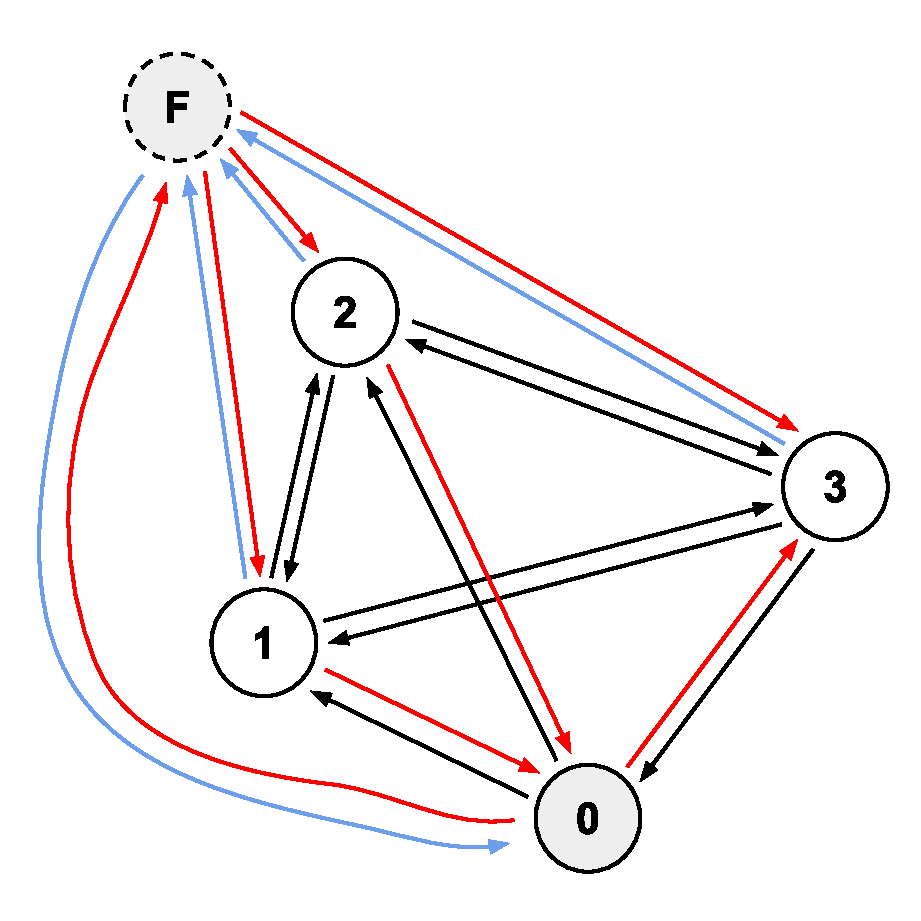
\includegraphics[width=0.4\textwidth]{./fig/photos/TSP.eps}
    \caption{An illustration of the modified distance matrix $\mathbf{D}_{mod}$ for the \ac{TSP} solver, that finds the optimal sequence of waypoints for each \ac{UAV}. 
    The vertex $v_{0}$ is the starting point of the sequence, vertices $\{v_{1}, v_{2}, v_{3}\}$ represent the waypoints to be visited by the \ac{UAV}, $v_{F}$ is an additional dummy virtual vertex. 
    The black edges represent the euclidean distance between corresponding vertices, the value of red edges is set to positive constant $M$, the value of blue edges is set to $0$. }
    \label{fig:tsp}
\end{figure}
%The modified distance matrix $\mathbf{D}_{mod}$ is then passed to the numerical solver.











\section{Path planning}
\begin{algorithm}
\caption{Multi-path planning}\label{alg:cap}
\begin{algorithmic}

\Function {plan\_paths}{$drones\_waypoints, drones\_poses$}
  \State $planned\_paths \gets \{\}$
  \For {$drone \in drones$} \Comment{iterate over drones based on priority}
    \State $obstacles \gets \{\}$
    \For {$path \in planned\_paths$}
      \State $obstacles \gets obstacles \cup \Call{inflate\_points}{path}$ %\Comment{mark positions around already planned paths as obstacles}
    \EndFor
    \State $path \gets \{\}$
    \State $segment\_start \gets drone\_pose$
    \For {$waypoint \in drone\_waypoints$}

      \If{ $waypoint \in obstacles$}
        \State \textbf{continue}
      \EndIf
      \State $path\_segment \gets \Call{astar\_planner}{start, waypoint, obstacles}$
      \State $segment\_start \gets waypoint$
      \State $path \gets path \cup path\_segment$
    \EndFor
    \State $planned\_paths \gets planned\_paths \cup path$
  \EndFor
  \State \Return $planned\_paths$
\EndFunction


\end{algorithmic}
\end{algorithm}






\subsection{Waypoint generation}
s a first step, the $\lambda$ matrix (containing the current estimate of sources position) is processed by a local maximum filter. 
The maximum filter works by sliding a window of a specified size over the $\lambda$.
The central position of the sliding window is highlighted as local maxima if it is greater than all other values in the sliding window.

Each waypoint (local maxima) is assigned with a weight $w$.
The weight is defined as follows:
\begin{equation}
  w_{j} = \frac{\lambda_{j}}{s_{j_{normalised}}}
\end{equation},
where $s_{j_{normalised}} = \frac{s_{j}}{\max_{J}( s_{j})}$ is a sensitivity value for given position $s_{j}$ divided by.
Such formulation of $w_{j}$ prioritise the points with the highest current estimate of ionizing radiation, that are less explored (have lower sensitivity).

\subsection{Task assignment}

To fasten the search time, the waypoints are divided among all the \ac{UAV}s involved in the experiment.
This is done by KMeans clustering method with minimum number of samples within each cluster.

The KMeans algorithm is an iterative clustering algorithm, that can divide data points into $k$ clusters.
Each cluster is represented with a virtual point called centroid, $c_{k}, k = 1, ... , K$, where $K$ is the number of clusters.
The algorithm proceeds as follows:

\begin{lstlisting}[caption={DroneDataMsg.msg (caption)}, title={Custom message for data sharing between \ac{UAV} and central unit.}, label={code1}]
Header header
geometry_msgs/Pose pose
geometry_msgs/Pose sensor_pose
geometry_msgs/PointStamped predicted_point
std_msgs/String status
\end{lstlisting}








\section{Finding an optimal sequence of waypoints for each \ac{UAV}}


\subsection{Path planning}




\section{Pipeline}

\begin{algorithm}
\caption{Planning pipeline}\label{alg:cap}
\begin{algorithmic}
  \State $POI \gets \Call{get\_points\_of\_interest}$
  \State $POI_{sorted} \gets \Call{filter\_points}{POI}$
  \State $POI_{exploration} \gets \Call{get\_unexplored\_area\_points}$
  
  \State $future\_poses \gets \Call{get\_future\_drone\_poses}$

  \State $W_{exploitation} \gets \Call{clustering}{future\_poses}$
  \State $W_{exploration} \gets \Call{clustering}{future\_poses}$
  
  \State
\end{algorithmic}
\end{algorithm}


collect more measurements
explore the least explored area

\subsection{Multirobotic approach}
there are two approaches - centralised and decentralised.
I use centralised.


